\documentclass[11pt,a4paper]{article}
\usepackage[T1]{fontenc}
\usepackage[utf8]{inputenc}
\usepackage[french]{babel}
\usepackage{lmodern,geometry,graphicx,booktabs,array,hyperref}
\geometry{margin=1.9cm}
\hypersetup{colorlinks=true,urlcolor=black,linkcolor=black}
\setlength{\parindent}{0pt}
\setlength{\parskip}{0.35em}
\renewcommand{\arraystretch}{1.16}

\begin{document}
\begin{center}
{\Large\bfseries Pipeline Big Data : données YouTube\par}
\vspace{0.25em}
{\large Rapport d'avancement -- semaine 2\par}
\vspace{0.55em}
Taha Hajji \quad Bouaicha Ibrahim \quad Ayoub Chenguir\\
Module Big Data Plateformes et Big Data Analytics
\end{center}

\section{Objectif et enchaînement des jobs}

Après la publication dans Kafka, l'objectif de la semaine 2 est de constituer un historique dans HDFS et d'en tirer de premiers indicateurs. La démonstration suit le chemin \texttt{Kafka $\rightarrow$ Spark $\rightarrow$ HDFS $\rightarrow$ Spark SQL}. Le traitement est lancé à la demande : le premier job lit les messages disponibles dans le topic au début de l'exécution, le second relit les fichiers Parquet produits. Cela correspond au jalon batch ; l'inférence en continu est prévue plus tard dans le projet.

Le topic \texttt{youtube.videos.raw} contient des messages JSON. Le job \texttt{kafka\_to\_hdfs.py} utilise le connecteur Kafka de Spark 3.5.3, avec les bornes \texttt{earliest} et \texttt{latest}. Il décode les messages selon un schéma explicite, vérifie que \texttt{video\_id} est présent et transforme les dates en horodatages Spark. Il conserve aussi le topic, la partition, l'offset et la date Kafka : ces colonnes permettent de revenir au message source en cas d'anomalie.

Les observations valides sont ajoutées sous \texttt{/data/youtube/bronze} en Parquet, avec une partition \texttt{collection\_date}. Le format Parquet évite de retraiter du JSON texte lors des analyses et garde le schéma des colonnes. Les DataNodes ont des volumes distincts et le facteur de réplication HDFS vaut 2.

\section{Indicateurs calculés}

Le job \texttt{indicators.py} lit la couche bronze. Il retire d'abord les doubles publications d'un même couple \texttt{(video\_id, collected\_at)}. Il choisit ensuite le relevé le plus récent pour chaque vidéo, afin de ne pas additionner plusieurs fois les vues d'une vidéo déjà collectée auparavant. Les sorties sont placées sous \texttt{/data/youtube/gold}.

\begin{center}
\small
\begin{tabular}{p{3.0cm}p{11.0cm}}
\toprule
Sortie & Contenu \\
\midrule
\texttt{channels} & Nombre de vidéos, vues totales observées, moyenne de vues et mentions J'aime par chaîne. \\
\texttt{published\_daily} & Nombre de vidéos et total des vues regroupés par date de publication. \\
\texttt{quality} & Nombre d'instantanés, nombre de vidéos distinctes et valeurs manquantes pour les vues et les mentions J'aime. \\
\bottomrule
\end{tabular}
\end{center}

La date de publication sert ici à regrouper les vidéos, mais les vues sont celles observées le jour de la collecte. Le total d'une ligne \texttt{published\_daily} ne mesure donc pas les vues gagnées ce jour-là. Cette distinction sera importante lorsque nous disposerons de plusieurs relevés réels.

\section{Exécution du parcours sur la fixture}

Le 9 novembre 2026, nous avons redémarré le cluster, publié les trois lignes fictives, lancé le job d'archivage puis le job d'indicateurs. Le premier job a annoncé \og Archived 3 valid Kafka events \fg{}. Le NameNode signalait deux DataNodes actifs et l'interface Spark deux workers actifs. La sortie HDFS confirme que les répertoires bronze et gold ont été créés.

\clearpage

\begin{figure}[htbp]
\centering
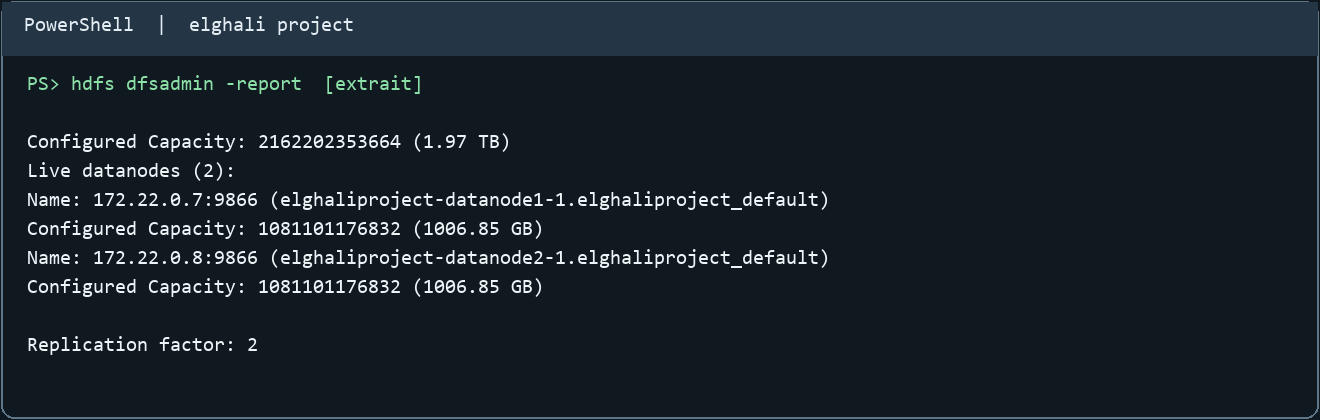
\includegraphics[width=0.75\linewidth]{docs/figures/terminal_hdfs_nodes.png}
\caption{Extrait de \texttt{hdfs dfsadmin -report} et valeur configurée de la réplication. Les deux DataNodes sont actifs.}
\end{figure}

\begin{figure}[htbp]
\centering
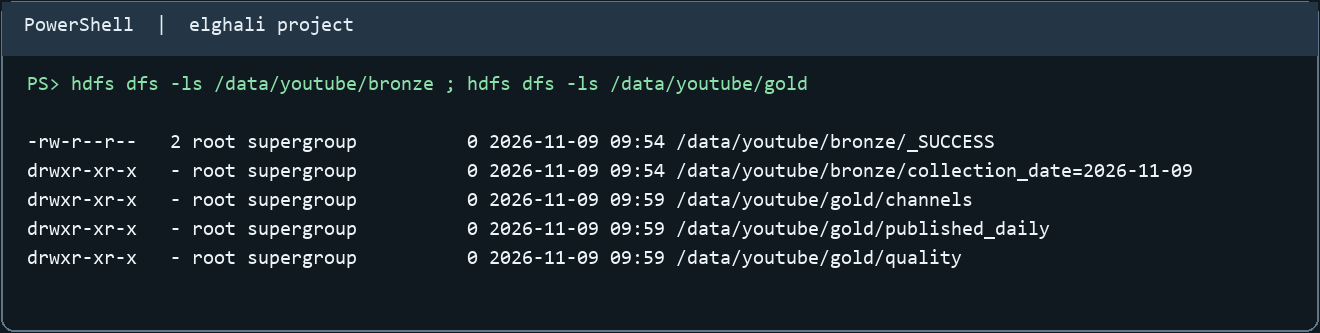
\includegraphics[width=0.75\linewidth]{docs/figures/terminal_hdfs_files.png}
\caption{Sorties de \texttt{hdfs dfs -ls} : partition bronze et trois dossiers d'indicateurs gold.}
\end{figure}

Le contrôle qualité donne trois instantanés pour trois vidéos distinctes. Les vues sont renseignées sur les trois lignes ; le nombre de mentions J'aime manque pour une vidéo. Ces chiffres correspondent exactement aux données de démonstration. La sortie \texttt{channels} donne 2\,150 vues pour les deux vidéos de \og Cours Data \fg{} et 2\,000 vues pour la vidéo de \og Data Lab \fg{}. Le total observé est donc de 4\,150 vues sur la fixture, sans signification statistique pour YouTube.

\begin{figure}[htbp]
\centering
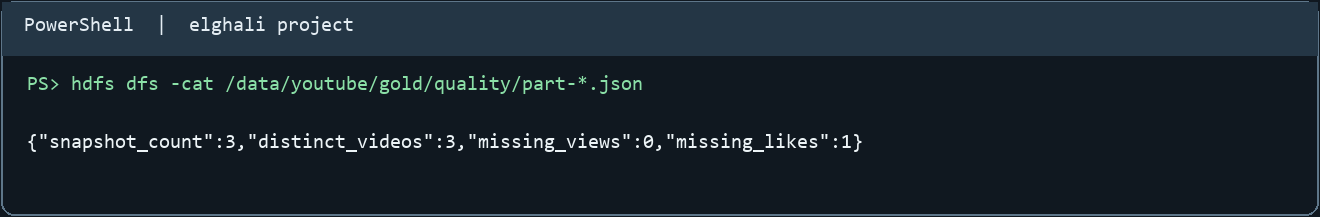
\includegraphics[width=0.72\linewidth]{docs/figures/terminal_quality.png}
\caption{Fichier JSON de contrôle qualité lu directement dans HDFS.}
\end{figure}

\section{Reproduction, limites et suite}

Le README fournit les commandes pour démarrer Compose, créer le topic, publier la fixture et lancer les deux \texttt{spark-submit}. Le connecteur Kafka de Spark a été chargé avec la version correspondant à Spark 3.5.3. Les fichiers bronze ont été vérifiés dans HDFS avec deux répliques. Après l'essai, les conteneurs peuvent être arrêtés avec \texttt{docker compose down} ; les volumes nommés conservent Kafka et HDFS pour une reprise.

Le job d'archivage ajoute les lignes à chaque relance. Si on le rejoue sur les mêmes offsets, des copies physiques sont créées, même si l'analyse les déduplique. Un suivi d'offsets ou un checkpoint sera nécessaire pour un fonctionnement durable. Un job de purge supprime les partitions de données API publiques âgées de plus de 30 jours ; les indicateurs doivent ensuite être recalculés. Enfin, les trois lignes fictives ne permettent ni de choisir une cible ML ni d'évaluer un modèle. Cette étape demandera des relevés réels datés et un découpage temporel adapté.

\section{Validation supplémentaire sur des données réelles}

Une fois la clé API disponible, nous avons d'abord vérifié la collecte sur une page de résultats. Nous avons ensuite élargi le lot avec les requêtes \og big data \fg{} et \og apache spark \fg{}. La première a fourni 529 vidéos et la seconde 471 vidéos supplémentaires après suppression des identifiants répétés. Le fichier local \texttt{data/youtube\_real.jsonl} contient donc 1\,000 vidéos distinctes pour environ 413~Ko. Les vues sont renseignées pour toutes les lignes ; 28 vidéos n'ont pas de nombre de mentions J'aime. Le plafond fixé à 1\,000 observations reste compatible avec les ressources du poste.

Pour ne pas mélanger les résultats avec la fixture, les 1\,000 observations ont été publiées dans le topic \texttt{youtube.videos.real}. Le job Spark les a archivées dans la couche bronze du dossier HDFS \texttt{youtube\_real} ; le second job a écrit les indicateurs dans la couche gold du même dossier. Le contrôle qualité HDFS confirme 1\,000 instantanés, 1\,000 vidéos distinctes, aucune vue manquante et 28 valeurs de mentions J'aime manquantes. Les fichiers Parquet de la couche bronze sont répliqués sur les deux DataNodes.

\begin{figure}[htbp]
\centering
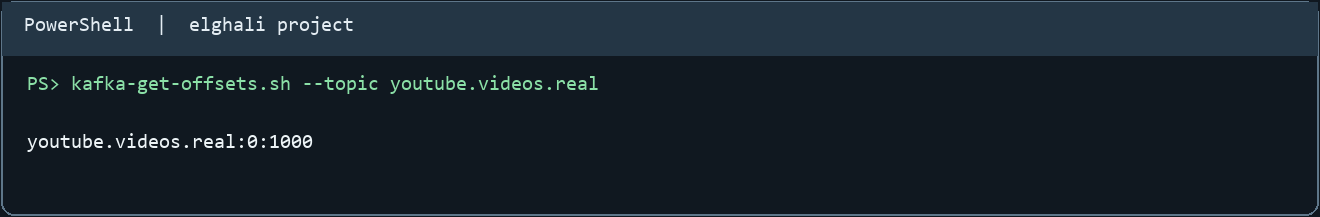
\includegraphics[width=0.72\linewidth]{docs/figures/terminal_real_kafka.png}
\caption{Offset final du topic réservé aux vidéos réellement obtenues par l'API.}
\end{figure}

\begin{figure}[htbp]
\centering
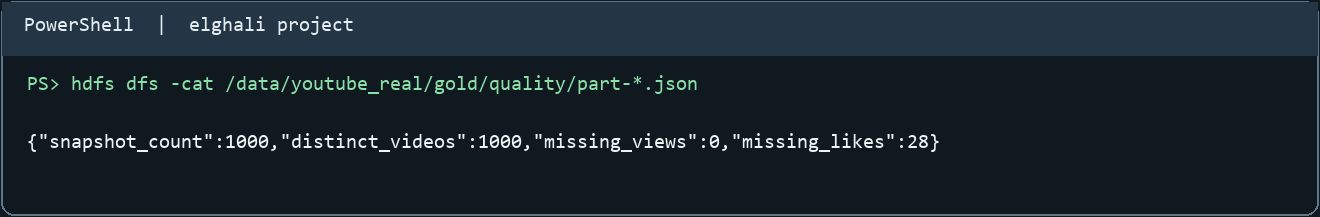
\includegraphics[width=0.75\linewidth]{docs/figures/terminal_real_quality.png}
\caption{Contrôle qualité du lot réel, lu dans la seconde zone HDFS.}
\end{figure}

Les deux recherches ont renvoyé des vidéos de 611 chaînes, publiées à des dates très différentes. Ce lot est utile pour vérifier l'ingestion et les calculs, mais il n'est pas représentatif d'une population bien définie. Pour la suite du projet, il faudra stabiliser la sélection des vidéos et refaire des relevés des mêmes identifiants afin de construire une cible de prédiction à horizon fixe. La validation du sujet par l'enseignante reste nécessaire.

\smallskip
{\small\textbf{Sources :} fiche de projet de Pr. El Ghali Btihal ;
\href{https://spark.apache.org/docs/3.5.3/structured-streaming-kafka-integration.html}{documentation Spark--Kafka} ;
\href{https://spark.apache.org/docs/3.5.3/sql-data-sources-parquet.html}{documentation Parquet} ;
\href{https://developers.google.com/youtube/terms/developer-policies}{règles de l'API YouTube}.}

\end{document}
